\documentclass{article}

\usepackage{amsthm}
\usepackage{amsmath}
\usepackage{amssymb}
\usepackage{graphicx}
\usepackage{epstopdf}
\usepackage{algorithm2e}
\usepackage{lineno}

\linenumbers
\theoremstyle{plain}
\newtheorem{thm}{Theorem}[section]
\newtheorem{prop}[thm]{Proposition}

\graphicspath{{./}{Figures}}

\begin{document}

% Title
\begin{center}
{\Large{Comparing Semi-Implicit and Full-Implicit Method for Solving Stiff Density Dependent Diffusion-Reaction Equations Arising in Biofilm Growth Models}}

\vspace{10pt}

{{Hermann J. Eberl and Eric M. Jalbert\\
  (heberl@uoguelph.ca, ejalbert@uoguelph.ca)\\}}
  
  {{Dept. of Mathematics and Statistics, University of Guelph,\\ 
  Guelph, ON N1G 2W1, Canada}}
\end{center}

\begin{abstract}
  Using the previously established mathematical model for the growth of \textit{Clostridium thermocellum} as an example, a comparison of a semi-implicit and fully-implicit numerical method will be conducted.
  This example is chosen specifically because it is a stiff problem.
  The semi-implicit method follows the idea of the semi-implicit Euler method.
  The fully-implicit method is similar except it computes the solutions multiple times for each time step, each using the newly computed values inplace of the solutions at the next time step.
  These two methods show a minute difference in accuracy, the fully-implicit method being mildly more correct.
  The difference in computational intensity is more pronouced, the semi-implicit method typically between 3 and 4 times faster. 
  The two values compare nicely and, given the correct situation, both have their uses.
  Ultimately, the gain in accuracy from the fully-impliciti method does generally justify the increase in accuracy; showing the semi-implici method as a sufficient numerical method for these types of problems.
\end{abstract}

\section{Intro}
  % Talk about basics of biofilms (should be more about C. Thermocellum)
  Bacterial biofilms are communities of microorganisms that adhere on immersed aquaeous surfaces that can support microbial growth based on the environmental conditions. 
  Biofilms are prevalent on both organic or inorganic surfaces in natural, industrial, or hospital settings.
  When attached to a surface, these bacterias embed themselves in a self-produced extracellular polymeric substance (EPS).
  The EPS provides a layer of protection against washout and biocides, making harmful biofilms difficult to remove.
  This attribute of biofilms is a problem since they are associated with medical issues in the form of, bacterial infections, dental plaque, and other diseases and industrial issues, such as biocorrosion of water pipes. 
  They also contribute positivly to wastewater treatment, groundwater protection, soil remediation, and other environmental engineering technologies.
  
  % Describe the history of modelling these systems.
  To further the understanding of biofilms, a diffusion-reaction model for biofilm growth was proposed in \cite{eberl2001deterministic}.
  This model is based on this work.
  
  % Talk about how to solve these systems.
  Through the use of some of many established numerical method, an analysis of this biological system can be completed.
  Typically, in these kind of time-dependent systems, one would discritize both space and time to facilitate obtaining the solution. 
  The numerical methods can be classified as explicit, semi-implicit, or fully-implicit based on the methods dependence for the state of the system.
  An explicit numerical method uses the current state of the system to compute the next state while a fully-implicit is the opposite \cite{butcher2008methods}.
  A semi-implicit method is specific to a system of differential equations, where at least one equation is solved using the current state and another is solved using the next state. 
  This difference between semi-implicit and fully-implicit numerical methods is that using a fully-implicit method is more computationally heavy, but gives greater accuracy.

  % Talk about the difference in what I'm doing here (i.e. that using a fully-implicit method won't add too much time but still be accurate, or that it doesn't matter which you use since there isn't a difference in accuracy). 
  

\section{Model}
  The specific biology that is discussed here is the growth of \textit{Clostridium thermocellum} biofilms on cellulose sheets.
  This cellulolytic anaerobic bacteria is a special type of biofilm, it displays uncharacteristic behaviour by not generating a EPS.
  Based on the work of \cite{dumitrache2014understanding}, a simple mathematical model to simulate the growth of \textit{C. thermocellum} can be created.
  They modelled the biomass density and nutrient concentration as a two PDE-coupled system. 
  Here the spatial diffusion of the nutrient concetration is removed to mimic the carbon substrait that \textit{C.Thermocellum} consumes to grow. 
  The PDE-ODE coupled system is purposed as,
  \begin{align} 
     M_t &= \nabla_x \left(  {D}(M) \nabla_x M \right) + {f}({C},M) M \label{equ:model_M}\\
     {C}_t &= -{g}({C}) M \label{equ:model_C}
  \end{align}
  where
  \begin{equation} \label{equ:model_D}
    {D}(M) = {\delta} \frac{M^\alpha}{(1-M)^\beta}
  \end{equation}
  \begin{equation} \label{equ:model_f}
    {f}({C},M) = {g}({C}) - \frac{y}{10} 
  \end{equation}
  \begin{equation} \label{equ:model_g}
    {g}({C}) = \frac{{y} {C}}{{k} + {C}}.
  \end{equation}
  
  The spatial diffusion of biomass $M$ is a density-dependent diffusion, given by (\ref{equ:model_D}).
  Here, $\delta$ depicts the diffusion rate of the biomass.
  The growth rate of biomass, ${f}({C},M)$, is given by (\ref{equ:model_f}). 
  The growth rate is Monod kinetic growth with a death term.
  There exists a yield term, $y$, that controls the amount of nutrients the biomass gains from the substraits. 
  In (\ref{equ:model_C}) there is only a consumption term from the bacteria consuming the carbon substrait. 
  Emphasis will be made to point out that (\ref{equ:model_C}) does not have spatial dependencies, since the cellulose sheet is a solid fiber that cannot move.
  
  \subsection {Nondimensionalization}
  For this system, it is better to nondimensionalize. To do this, the following variable changes are used:
  \begin{align}
    x &= \frac{\chi}{L} \implies L dx = d\chi\\
    t &= \mu \tau \implies \frac{1}{\mu} dt= d\tau\\
    C &= \frac{\overline{C}}{C_0} \\
    \delta &= \frac{1}{\mu L^2} \overline{\delta} \\
    k &= \frac{\overline{k}}{C_0} \\
    \nu &= \frac{\overline{\nu}}{\mu C_0} \\
    \mu &= \overline{\mu}
  \end{align}
  This gives the system
  \begin{align}
    M_t &= \frac{1}{\mu L^2} \nabla_x \left(\hat{D}(m) \nabla_x M \right) + \frac{1}{\mu} \hat{f}(C,M) \\
    C_t &= \frac{ -1}{C_0 \mu} \hat{g}(C,M)
  \end{align}
  
  where 
  \begin{equation}
    \hat{D}(M) = {\mu L^2 \delta} \frac{M^\alpha}{(1-M)^\beta}
  \end{equation}
  
  \begin{equation}
    \hat{f}({C},M) = \frac{{\mu} {C C_0}}{{k C_0} + {C C_0}} M \left(1 - \left( \frac{M}{{C}} \frac{M_0}{C_0} \right)^\gamma \right) \\
  \end{equation}
  
  \begin{equation}
    \hat{g}({C},M) = -\frac{{\mu C_0 \nu} {C C_0}}{{k C_0} + {C C_0}} M \\
  \end{equation}
  
  This can be greatly simplified by cancelling out parameters.
  
  \begin{align}
    M_t &= \nabla_x \left( {\delta} \frac{M^\alpha}{(1-M)^\beta} \nabla_x M\right) + \frac{ C }{{k } + {C}} M \left(1 - \left( \frac{M}{{C}} \frac{M_0}{C_0} \right)^\gamma \right) \\
    C_t &= - \frac{\nu C}{k + C} M
  \end{align}
  
  Now we can name functions and get the final nondimensionalized system.
  
  \begin{align} \label{equ:model_system}
    M_t &= \nabla_x \left( D(M) \nabla_x M \right) + f(C,M) \\
    C_t &= - g(C,M) 
  \end{align}
  
  where
  
  \begin{equation}
  \begin{aligned} \label{equ:model_functions}
    D(M) &= \delta \frac{M^\alpha}{(1 - M)^\beta} \\
    f(C,M) &= \frac{ C }{{k } + {C}} M \left(1 - \left( \frac{M}{{C}} \frac{M_0}{C_0} \right)^\gamma \right) \\
    g(C,M) &= \frac{\nu C}{k +C} M
  \end{aligned}
  \end{equation}
  
  % Talk about what each function represents, and what each equation is. 
  % Also mention the significance of each parameter  if possible.

  This system is solved on a non-dimensionalized square region $\Omega \in \left[0,1 \right] \times \left[0,1 \right]$.
  On this region, there are Neumann boundary conditions defined as
  \begin{equation}
    \frac{\partial M}{\partial x} = \frac{\partial C}{\partial x} = 0, \quad \text{on } \partial\Omega. 
  \end{equation}

\section{Method}
  There are three main aspects to the numerical method of solving this system.
  The system must be temporally and spatially discritized, then a solution for $C$ and $M$ can be computed using numerical methods.
 
  For the solution of $C$, since it has no spatial diffusion, a simple application of the Trapezidral rule can be used.
  The idea is to integrate both sides of (\ref{equ:model_C}) to get,
  \begin{equation} \label{equ:ctrapizodal}
    C^{n+1} - C^{t_n} = \frac{t_{n+1} - t_{n}}{2} \left( g(C^{n+1}, M^{t_{n+1}}) + g(C^{t_n}, M^{t_n}) \right).
  \end{equation}
  By rearranging (\ref{equ:ctrapizodal}) and subbing in (\ref{equ:model_g}) an equation explicitly for $C_{t_{n+1}}$ is found.
  This solution gives two values for $C_{t_{n+1}}$ since it is solved using the quadratic formula.
  Only the positive branch of the quadratic formula is relavent to this problem, since the negative branch behaves unrealisticly.
  
  The solution of $M$ is more involved, because of the density-dependent diffusion term.
  This means that it must be spatially discritized as well as temporally discritized. 
  The spatial discritization of the system is a simple application of the finite difference method.
  Following the example of finite differences for 2-D problems as described in \cite{saad2003iterativeMethod} a grid is created to approximate each point using a five-point stencil.
  Here, the values at the boundaries are unknown and as such are also included in the five-point stencil
  These boundary points are computed using a second order appoximation.
  The temporal discritization is a forward difference between the current and next time step.
  Applying these discritizations to (\ref{equ:model_M}) and rearranging gives a system of linear equation defined by,
  \begin{equation} \label{equ:discritizeM}
  \begin{aligned}
    \frac{M^n_{i,j}}{\Delta t} &= \frac{-D^n_{i,j-\frac{1}{2}}}{\Delta y ^2} \cdot M^{n+1}_{i,j-1} + \frac{-D^n_{i-\frac{1}{2},j}}{\Delta x ^2} \cdot M^{n+1}_{i-1,j}  \\
    &  +  \left[ \frac{D^n_{i,j-\frac{1}{2}}}{\Delta y ^2} + \frac{D^n_{i-\frac{1}{2},j}}{\Delta x ^2} + \frac{D^n_{i+\frac{1}{2},j}}{\Delta x ^2} + \frac{D^n_{i,j+\frac{1}{2}}}{\Delta y ^2} - f(C^n, M^n) + \frac{1}{\Delta t} \right] \cdot M^{n+1}_{i,j}  \\
    &  + \frac{-D^n_{i+\frac{1}{2},j}}{\Delta x ^2} \cdot M^{n+1}_{i+1,j} + \frac{-D^n_{i,j+\frac{1}{2}}}{\Delta y ^2} \cdot M^{n+1}_{i,j+1},
  \end{aligned}
  \end{equation} 
  where $M^n_{i,j} = M^{t_n}(x_i,y_j)$, $D^n_{i,j} = D(M^n_{i,j})$, and $(x_i,y_j)$ is the ordered pair at grid point $i,j$.
  
  Using (\ref{equ:discritizeM}) a five-diagonal block matrix can be created, defined as,
  \begin{equation} \label{equ:five_diagonal_matrix_M}
    A = 
    \left( 
      \begin{array}{c c c c c c c c c c}
        M_{i,j} & M_{i+1,j} &  & M_{i,j+1} &   \\
        M_{i-1,j} & \ddots & \ddots &   &  \ddots &   \\
        & \ddots & \ddots & \ddots & & \ddots & \\
        M_{i,j-1} &  & M_{i-1,j} & M_{i,j} & M_{i+1,j} &   &  M_{i,j+1} &   \\
        & \ddots & & \ddots & \ddots & \ddots & & \ddots\\
        & & M_{i,j-1} &  & M_{i-1,j} & M_{i,j} & M_{i+1,j} &  & M_{i,j+1} \\
        & & & \ddots & & \ddots & \ddots & \ddots & \\
        & & & & \ddots & & \ddots & \ddots & M_{i+1,j} \\
        & & & & & M_{i,j-1} & & M_{i-1,j} & M_{i,j}
      \end{array}
  %      \begin{array}{c c c c c c c c c c}
  %        M_{i,j} & M_{i+1,j} & \cdots & M_{i,j+1} &  \cdots \\
  %        M_{i-1,j} & M_{i,j} & M_{i+1,j} &  \cdots &  M_{i,j+1} &  \cdots \\
  %        \cdots &  M_{i-1,j} & M_{i,j} & M_{i+1,j} &  \cdots &  M_{i,j+1} &  \cdots \\
  %        & & \ddots & \ddots & \ddots & & \ddots & \\
  %        M_{i,j-1} &\cdots & \cdots & M_{i-1,j} & M_{i,j} & M_{i+1,j} &  \cdots &  M_{i,j+1} &  \cdots \\
  %        & \ddots & & & \ddots & \ddots & \ddots & & \ddots\\
  %        & \cdots &M_{i,j-1} & \cdots& \cdots & M_{i-1,j} & M_{i,j} & M_{i+1,j} & \cdots & M_{i,j+1} \\
  %        & & \cdots & M_{i,j-1} &  \cdots &\cdots & M_{i-1,j} & M_{i,j} & M_{i+1,j} & \cdots\\
  %        & & & \cdots & M_{i,j-1} &  \cdots &\cdots & M_{i-1,j} & M_{i,j} & M_{i+1,j} \\
  %        & & & & \cdots& M_{i,j-1} &  \cdots &\cdots & M_{i-1,j} & M_{i,j}\\
  %      \end{array}
    \right),
  \end{equation}
  where each $M_{i,j}$ is the coefficient based on (\ref{equ:discritizeM}).
 
  The solving of (\ref{equ:five_diagonal_matrix_M}) can be completed through use of a linear solver. 
  According to \cite{barret1987templates}, if (\ref{equ:five_diagonal_matrix_M}) is positive definite and symmetric then it can be solved using the Conjugate Gradiant method.
  \begin{prop}
    The matrix $A$, defined in (\ref{equ:five_diagonal_matrix_M}), is positive definite and symmetric.
  \end{prop}
  \begin{proof}
    Matrix $A$ is positive definite if all the eigenvalues are positive. 
    Using Ger{\v s}gorin's circle theorem, see \cite{gerschgorin1931uber_die_abgrenzung}, the eigenvalues can be shown to be positive if, on all rows independently, the sum of the off-diagonals values are less then the diagonal value.
    Mathematically we have,
    \begin{equation}
      \begin{aligned}
      & \left| \frac{-D^n_{i,j-\frac{1}{2}}}{\Delta y ^2} + \frac{-D^n_{i-\frac{1}{2},j}}{\Delta x ^2} + \frac{-D^n_{i+\frac{1}{2},j}}{\Delta x ^2} + \frac{-D^n_{i,j+\frac{1}{2}}}{\Delta y ^2} \right| \\
      &\quad < \left| \frac{D^n_{i,j-\frac{1}{2}}}{\Delta y ^2} + \frac{D^n_{i-\frac{1}{2},j}}{\Delta x ^2} + \frac{D^n_{i+\frac{1}{2},j}}{\Delta x ^2} + \frac{D^n_{i,j+\frac{1}{2}}}{\Delta y ^2} - f(C^n, M^n) + \frac{1}{\Delta t} \right|, 
      \end{aligned}
    \end{equation}
    which simplifies to,
    \begin{equation}
      f(C^n_{i,j}, M^n_{i,j}) < \frac{1}{\Delta t},
    \end{equation}
    which is true give the values of $\Delta t$ that are used. Therefore we have that $A$ is positive definite.

    The symmetry of $A$ can be trivially shown if one considers the formation of the diagonals.
    On a single row, each element corresponds to the adjacent grid points of grid $i,j$.
    As the grid ordering counts along, the elements that are equidistance from the diagonal are actually reference to the same grid point. 
    Therefore we have symmetry. \qed
  \end{proof} 

  Given that $A$ is positive definite and symmetric, the conjugate gradiant method can be used to compute the solution.
  As an added property, $A$ also happens to be diagonally dominate.
  This means that it could be solved using Bi-Conjugate Gradient Method.
  However the Conjugate Gradient method has a faster computation time then Bi-Conjugate Gradiant method for this problem and is used for this reason \cite{barret1987templates}.

  Now that the method for solving $C$ and $M$ have been discussed, the method for solving the system as a whole can be investigated. 
  Since $M^{t_{n+1}}$ only depends on $C^{t_n}$ and $M^{t_n}$ while $C^{n+1}$ depends on $C^{t_n}, M^{t_n},$ and $M^{t_{n+1}}$ the solution for $M$ should be computed first and then it can be used to compute $C$. 
  This idea is translated into Algorithm \ref{alg:iterateCM} to be the fully-implicit method for solving the system.
  The semi-implicit method for solving the system is the same as Algorithm \ref{alg:iterateCM} but with $eSoln = 0$, forcing only a single iteration of the loop.

  \begin{algorithm}[h!tb]
    \KwData{$M_{prev}$ and $C_{prev}$ is previous timestep solutions}
    \Begin
    {
      \While{diffC $>$ eSoln $and$  diffM  $> $ eSoln}
      {
          Solve for $M^{i+1}$ using $C^{i}$ and $M_{prev}$\;
          Solve for $C^{i+1}$ using $C_{prev}$, $M^{i+1}$, and $M_{prev}$\;
          Let diffC $=  (C^{i+1} - C^i)$\;
          Let diffM $= (M^{i+1} - M^i)$\;
          Let $C^{i} = C^{i+1}$
          Let $M^{i} = M^{i+1}$\;
      }
    }
    \caption{Algorithm for the fully-implicit solving of (\ref{equ:model_M}-\ref{equ:model_C}).}
    \label{alg:iterateCM}
  \end{algorithm}

  % Probably mention that it's stored in a diagonal format.


\section{Results}
  \subsection{Simulation Setup}
    All the simulations were run on a custom built workstation with an Intel Xeon CPU E5-2650 (1.2 GHz, 20 MB cache size) and 32 GB RAM under Red Hat Enterprise Linux Server release 6.5 (Santiago). 
    Running the simulations with OpenMP, took advantage of the 16 processers of the Intel Xeon CPU, each with 2 threads. 
    The GNU fortran compiler version 4.4.7 was used for the typical simulation results; compiler arguments were \begin{verbatim} -O3 -fdefault-real-8 -fopenmp .\end{verbatim}
    The Intel Fortran compiler version 14.0.2 was used for the speed results; compiler arguments were \begin{verbatim} -O3 -r8 -openmp. \end{verbatim}

    The simulations were solved on a $1024 \times 1024$ grid, using $\Delta t = 10^{-2}$.
     
     % If it's completed and works, talk about the openACC use here.
  
  \subsection{Results}
    Using the parameter values defined in the Appendix, the simultation was run and the results were as shown in Figure \ref{fig:typical_simulation_results}.

    % Show a few snap shots of the map view?
    \begin{figure}[h!tb]
      \begin{center}
      \begin{tabular}{c c}
        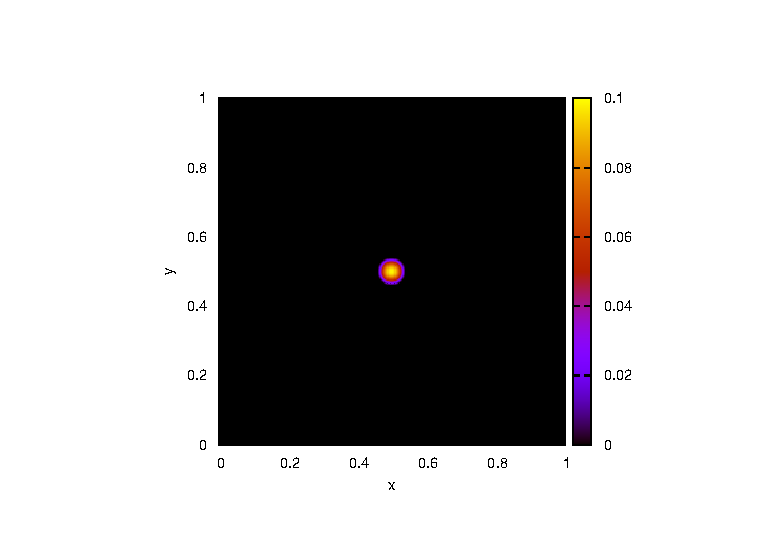
\includegraphics[scale = 0.5]{typicalSim-t0.eps}&
        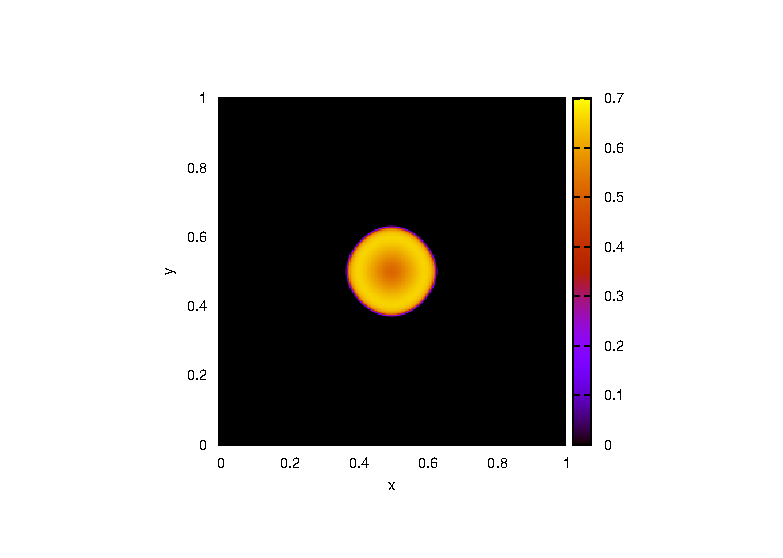
\includegraphics[scale = 0.5]{typicalSim-t10.eps}\\
        (a) & (b) \\
        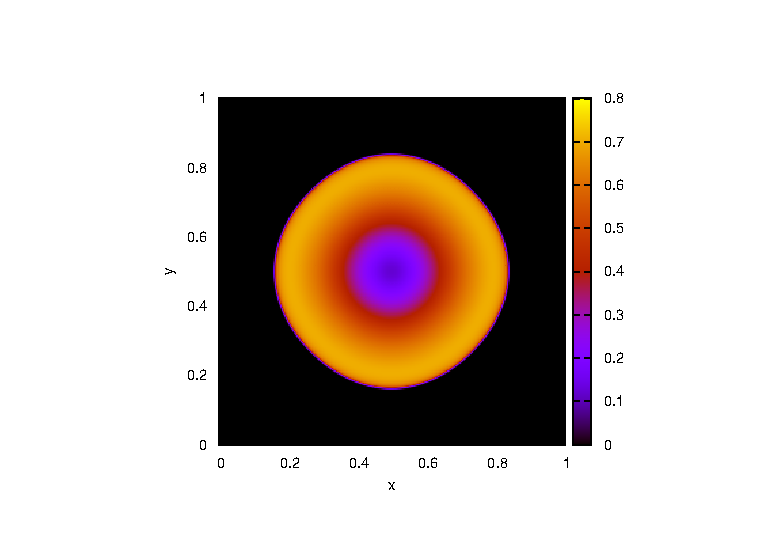
\includegraphics[scale = 0.5]{typicalSim-t20.eps}&
        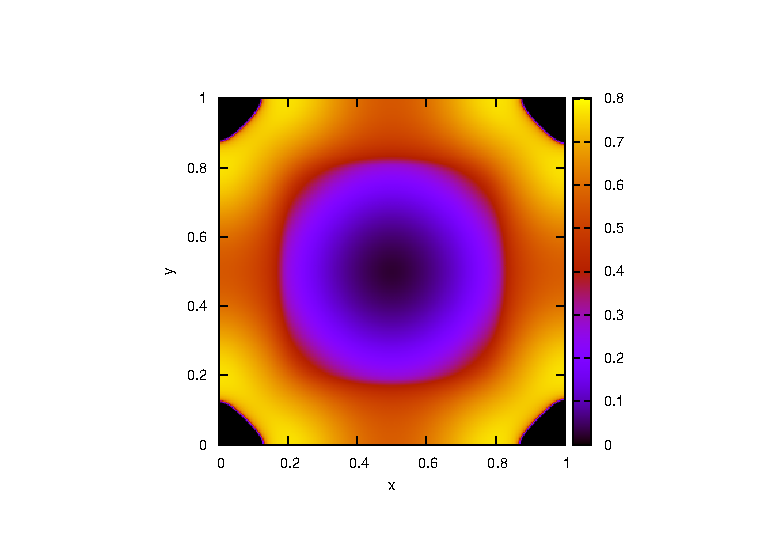
\includegraphics[scale = 0.5]{typicalSim-t30.eps}\\
        (c) & (d) \\
      \end{tabular}
      \caption{Typical simulation using parameters from Appendix at (a) $t = 0$, (b) $t = 10$, (c) $t = 20$, (d) $t = 30$}
      \label{fig:typical_simulation_results}
      \end{center}
    \end{figure}
    % Describe, biologically, what the soltion shows?

  \subsection{Comparisons}
    % Also mention the Accuracy of the solutions by using the norm of each solution compared to the  most accurate one.... (Maybe take a solution at a higher grid resolution?, not sure what to do here)
    A comparison of the the two methods can be done by looking at both their computation time and the accuracy of the solution.
    The computation time is computed by the system clock from the start of the algorithm to the end of the algorithm. 
    The accuracy of the solution can be found by computing the normed-difference between two solutions, as follows,
    \begin{equation}
      \epsilon_{sol} = \frac{||u_1 - u_2||}{||u_1||}
    \end{equation}
    Two comparisons will be done with the norm. 
    One with the solution at the current grid size and the solution at the next smallest grid size.
    This is because, the samller the grid refinement, the more accurate the solution. 
    Thus to compare the accuracy of methods, this will be used.
    The other will be with the solution and the solution with the smallest $eSoln$, as defined in Algorithm \ref{alg:iterateCM}.
    These two comparison will provide two difference measures of the accuracy of the method.

    The other comparison will be with where the method is spending its time.
    The fully-implicit method should have less iterations of the linear solver.
    Thus with will be measured as $Iteration 2$. 
    $Iterations 1$ is the number of iterations between solving $M$ and $C$, according to Algorithm \ref{alg:iterateCM}.
    
    The results of the method comparison can be seen in Tabel \ref{tab:tolerance_comparison}.
    
    \begin{table}[h!tb]
      \begin{center}
      \begin{tabular}{|c|c|c|c|c|c|c|}
        \hline
        Tol. 1 & Computation Time & $\epsilon_{sol}$ & Avg. Iter. 1 & Max Iter. 1 & Avg. Iter. 2 & Max Iter. 2 \\
        \hline
        $10^{0}$ & 1430.05 & ---- & 1 & 1 & 44.08 & 72 \\
        $10^{-2}$ & ---- & ---- & ---- & ---- & ---- & ---- \\
        $10^{-4}$ & ---- & ---- & ---- & ---- & ---- & ---- \\
        $10^{-8}$ & ---- & ---- & ---- & ---- & ---- & ---- \\
        \hline
      \end{tabular}
      \caption{Results from running simulation with different Tolerance 1 values. Note, Tolerance 1 of $10^{0}$ is the semi-implicit method.}
      \label{tab:tolerance_comparison}
      \end{center}
    \end{table}

\section{Conclusions}
  The numerical simultating of this problem can be solved in many differenct manners.
  Using the fully-implicit method as described in Algorithm \ref{alg:iterateCM} allows for an extra degree of accuracy for the solution.
  That being said, the difference in computation time is not neccessarily worth the increased workload.
  The semi-implicit method has shown to provide solution that are sufficiently accurate and thus the extra computations for the fully-implicit method are not always needed.
  The choice of method is mostly dependent on the problem that is being solved and the required accuracy of the solution.
  With powerful computers becoming more readily available, the sacrifice of computation speed becomes a smaller price.


\section*{Appendix}
  \begin{table}[h!bt]
    \centering
    \begin{tabular}{|c | l | l|}
      \hline 
      Variable/Parameter & Dimensions & Parameter Value\\
      \hline 
      $x$ & [$days$] & $-$ \\
      $t$ & [$meters$] & $-$ \\
      $ M  $ & [$-$] & $-$\\
      $ C  $ & [$\frac{grams}{meters^3}$]  & $-$\\
      $ {\delta} $ & [$\frac{meters^2}{days}$] & $10^{-12}$ \\
      $ \alpha $ & [$-$] & $4$\\
      $ \beta  $ & [$-$] & $4$\\
      $ {y}$ & [$days^{-1} $] & $6$ \\
      $ {k}  $ & [$\frac{grams}{meters^3}$] & $4$ \\
     % $ \gamma $ & [$-$] & $0.5$\\
     % $ {\nu}$ & [$\frac{grams}{meters^3 \cdot days}$] & $\frac{\mu M_0}{0.63}$ \\
     % $ M_0 $ & [$-$] & $10000$ \\
     % $ C_0 $ & [$\frac{grams}{meters^3}$]  & $30$ \\
      \hline
    \end{tabular}
    \caption{List of parameters and their dimensions}
        \label{tab:varDimensions}
  \end{table}

\newpage

\bibliographystyle{plain}
\bibliography{References}


\end{document}
